%travail_visitor
\subsection{Visiteur}
\begin{figure}[h]
\begin{center}
    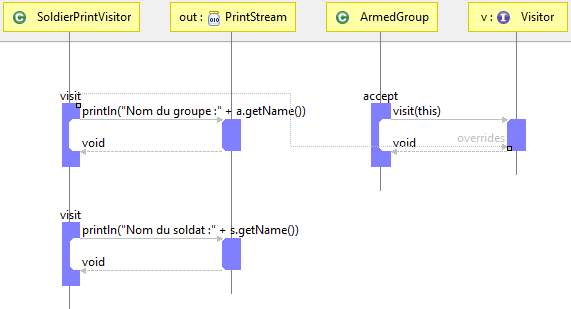
\includegraphics[width=11cm]{diagSeqVisitor}
\end{center}
    \caption{Diagramme de séquence du pattern visiteur}
    \label{sequence-visiteur}
\end{figure}

Nous avions à la fois des groupes armés ainsi que des soldats de différentes catégories. Afin de faciliter l'ajout de nouvelles fonctionnalités à la fois sur les groupes armés et sur les soldats, nous avons mis en place le pattern \emph{Visiteur}. Sans ce pattern, à chaque ajout de fonctionnalités, nous étions obligés de rajouter les méthodes dans nos classes \emph{Horseman}, \emph{Infantry} et \emph{ArmedGroup}, d'autant plus si nous voulions faire des traitement différents en fonction de chaque classe. Grâce au pattern \emph{Visiteur}, l'ajout de fonctionnalités supplémentaires (comme l'affichage de tous les soldats formant un groupe armé ou le comptage des effectifs de soldats par rapport à leur type au sein d’un groupe armé) se fait maintenant dans une seule classe, sans avoir à toucher le reste du code. Nous avons créé une classe \emph{SoldierPrintVisitor} pour ajouter la fonction d'affichage des soldats ainsi que la classe \emph{SoldierCountVisitor} pour ajouter la fonction de comptabilisation. Vous pouvez voir un exemple du déroulement des appels de méthodes en figure \vref{sequence-visiteur}. Tout ceci est totalement transparent vis-à-vis du reste du code : c'est là tout l'intérêt du pattern \emph{Visiteur}. On n'applique donc qu'un nombre minimal de modifications sur les autres classes de l'application et nous avons la possibilité de faire des traitements spécifiques pour chacune des classes de l'application. En résumé, nous pouvons maintenant ajouter des fonctionnalités sur les objets de notre choix sans toucher au reste du code.